\documentclass{article}
\usepackage{polski}
\usepackage[utf8]{inputenc}
\usepackage{mathtools}
\usepackage{graphicx}

\graphicspath{{img/}}

\begin{document}

\section{Hyperball vs Hypercube}


\subsection{Volume of hyperball:}
for n = 2k

\begin{equation}
  V_{2k}(R) = \dfrac{\pi^{2k}}{k!}R^{2k}
\end{equation}

for n = 2k + 1

\begin{equation}
  V_{2k+1}(R) = \dfrac{2(k!){(4\pi)}^{k}}{(2k+1)!}R^{2k+1}
\end{equation}

\subsection{Volume of hypercube:}

for hyper cube with edge length of 'a':

\begin{equation}
  V_{n}(a) = a^n
\end{equation}

\subsection{Answer}

a = 2.0 and R = 1.0 :

\subsubsection{n = 2k}

\begin{equation}
  \dfrac{Hyperball \quad volume}{Hypercube \quad Volume} * 100\% =  \dfrac{\pi^{2k}}{k!2^{2k}} * 100\%
\end{equation}

\subsubsection{n = 2k + 1}

\begin{equation}
  \dfrac{Hyperball \quad volume}{Hypercube \quad Volume} * 100\% =  \dfrac{k!{\pi}^{2k}}{(2k+1)!}} * 100\%
\end{equation}

\subsection{Experimental results: Percentage of points in hypercube}

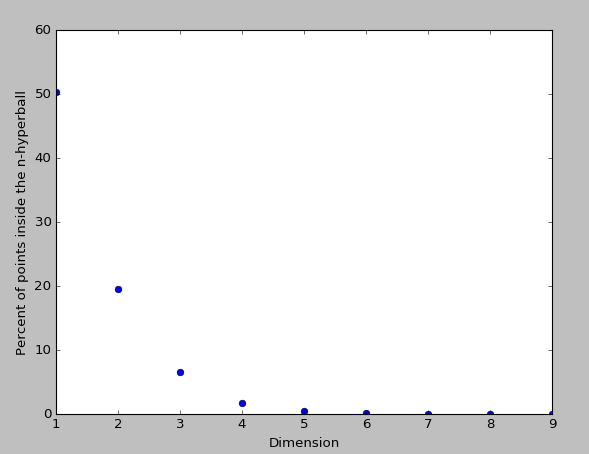
\includegraphics[width=\textwidth]{points}

\subsubsection{Discussion}

The plot shows that the percentage of point that fall into the hypercube decreases exponentially. Which
yields two main conclusions: human intuition isn't a good tool in high dimension hyperspace and secondly
the number of point in a randomly choses neighbourhood drops dramatically.

\section{CoD and k-NN}

The k-nearest neighbours rule requires the neighbours to be a reasonably good representative of the neighbourhood of the query point (they need to be relatively close to the query point).
Because the volume in hyperspace increases exponentially with the number of dimensions, data points density drops significantly, therefore the points are less likely to be in the near neighbourhood of the query point. In effect k-NN doesn't perform well.

\subsubsection{Experimental results: Ratio of std to average value}

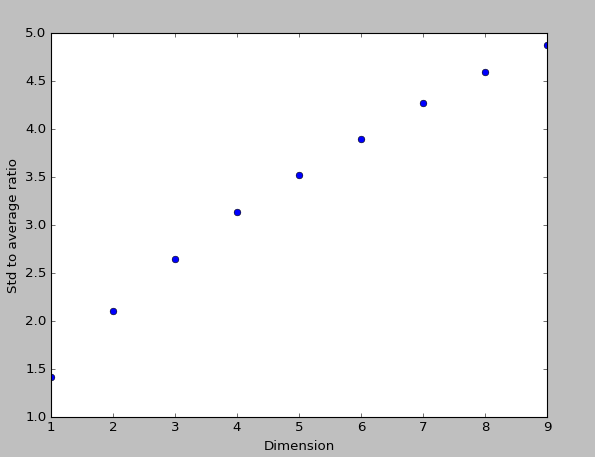
\includegraphics[width=\textwidth]{std_to_average_ratio}

\subsubsection{Discussion}

From the plot above one could conclude that in high dimension space the ratio of std to average distance grows very slowly,
which means that an euclidean distance is no loger a viable tool for comparing datapoints in high dimension hyperspace.


\end{document}
